%\documentstyle[epsf,twocolumn]{jarticle}       %LaTeX2e仕様
\documentclass[twocolumn]{jarticle}     %pLaTeX2e仕様(platex.exeの場合)
% \documentclass[onecolumn]{ujarticle}   %pLaTeX2e仕様(uplatex.exeの場合)
%%%%%%%%%%%%%%%%%%%%%%%%%%%%%%%%%%%%%%%%%%%%%%%%%%%%%%%%%%%%%%
%%
%%  基本バージョン
%%
%%%%%%%%%%%%%%%%%%%%%%%%%%%%%%%%%%%%%%%%%%%%%%%%%%%%%%%%%%%%%%%%
\setlength{\topmargin}{-45pt}
%\setlength{\oddsidemargin}{0cm}
\setlength{\oddsidemargin}{-7.5mm}
%\setlength{\evensidemargin}{0cm}
\setlength{\textheight}{24.1cm}
%setlength{\textheight}{25cm}
\setlength{\textwidth}{17.4cm}
%\setlength{\textwidth}{172mm}
\setlength{\columnsep}{11mm}

%\kanjiskip=.07zw plus.5pt minus.5pt


% 【節が変わるごとに (1.1)(1.2) … (2.1)(2.2) と数式番号をつけるとき】
%\makeatletter
%\renewcommand{\theequation}{%
%\thesection.\arabic{equation}} %\@addtoreset{equation}{section}
%\makeatother

%\renewcommand{\arraystretch}{0.95} 行間の設定
%%%%%%%%%%%%%%%%%%%%%%%%%%%%%%%%%%%%%%%%%%%%%%%%%%%%%%%%
%\usepackage{graphicx}   %pLaTeX2e仕様(\documentstyle ->\documentclass)
\usepackage[dvipdfmx]{graphicx}
\usepackage{subcaption}
\usepackage{multirow}
\usepackage{amsmath}
\usepackage{url}
\usepackage{ulem}
\usepackage{algorithm}
\usepackage{algorithmic}
\usepackage{listings} %,jlisting} %日本語のコメントアウトをする場合jlistingが必要
%ここからソースコードの表示に関する設定
\lstset{
  basicstyle={\ttfamily},
  identifierstyle={\small},
  commentstyle={\smallitshape},
  keywordstyle={\small\bfseries},
  ndkeywordstyle={\small},
  stringstyle={\small\ttfamily},
  frame={tb},
  breaklines=true,
  columns=[l]{fullflexible},
  numbers=left,
  xrightmargin=0zw,
  xleftmargin=3zw,
  numberstyle={\scriptsize},
  stepnumber=1,
  numbersep=1zw,
  lineskip=-0.5ex
}
%%%%%%%%%%%%%%%%%%%%%%%%%%%%%%%%%%%%%%%%%%%%%%%%%%%%%%%%
\begin{document}

	%bibtex用の設定
	%\bibliographystyle{ujarticle}

	\twocolumn[
		\noindent
		\hspace{1em}
		2020 年 10 月 2 日
		ゼミ資料
		\hfill
		B4 杉山 竜弥
		\vspace{2mm}

		\hrule
		\begin{center}
			{\Large \bf 進捗報告}
		\end{center}
		\hrule
		\vspace{9mm}
	]

	% ‚ここから 文章 Start!
% \section{今週やったこと}
% \begin{itemize}
% 	\item グラフ距離の計算
% \end{itemize}

\section{問題}
ショートカットの数を固定していたため, ベースラインが探索空間に入っていなかった.
そこでショートカット数も学習に加えた.

ブロックの定義にショートカット数$\beta$を加え,
\begin{equation}
  \label{equ:cut}
  x_i = {\rm ConvBn}_{i}(x_{i-1}) + \beta_i * \sum_j \alpha_{ij} * {\rm shortcut}_{ij} (x_j)
\end{equation}
のように変えた.
そのまま学習すると, $\beta=0$で勾配の更新ができなくなるので,
\begin{equation}
  \label{equ:cut}
  \hat{\beta} = \begin{cases}
    \exp(\beta - 1) & (\beta \leq 1) \\
    \log(\beta) + 1 & (otherwise)
  \end{cases}
\end{equation}
指数関数で値域を0より大きくした$\hat{\beta}$(初期値1)を使用する. $\log$は特に理由はない

\section{実験}

\begin{table}[tb]
  \begin{center}
    \caption{実験の設定}
    \begin{tabular}{|c|c|} \hline
      model & VGG19 \\ \hline
      Optim(model) & SGD(lr=0.01, momentum=0.9) \\ \hline
      Optim($\alpha$) & Adam(lr=0.005, $\beta$=(0.5, 0.999)) \\ \hline
      Loss & Cross Entropy Loss \\ \hline
      dataset & cifar10 \\ \hline
      batch size & 64 \\ \hline
      train data & 25000 + 25000 / 25000 \\ \hline
      epoch & 50 / 100 \\ \hline
    \end{tabular}
    \label{tab:setting}
  \end{center}
\end{table}

表\ref{tab:setting}に実験設定を示した.
ショートカット関数はstrideありのとき, Factorized Reduceを使う.
% ただしstrideが大きいときに対応する関数がないため2より大きい辺を削除した.

評価段階では$\hat{\beta}$の小数点を丸めて整数にし, $\alpha$の上位から順にショートカットを選んでグラフとした.

(評価段階のデータサイズを間違えて25000で学習してしまった.)

\subsection{結果}

\begin{table}[tb]
  \begin{center}
    \caption{Accuracyの比較}
    \begin{tabular}{|c||c|c|c|} \hline
       & accuracy(\%) & 学習時間 & データ数 \\ \hline \hline
      探索 & 88.24 & 50 & 50000 \\ \hline
      評価 & 87.96 & 100 & 25000 \\ \hline
      ベースライン & 87.96 & 100 & 25000 \\ \hline
    \end{tabular}
    \label{tab:acc}
  \end{center}
\end{table}


\begin{figure}[tb]
	\begin{center}
		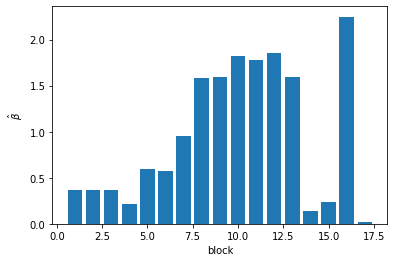
\includegraphics[clip,width=75mm]{beta.png}
		\caption{探索後の$\hat{\beta}$の値}
		\label{fig:beta}
	\end{center}
\end{figure}

\begin{figure*}[tb]
	\begin{center}
		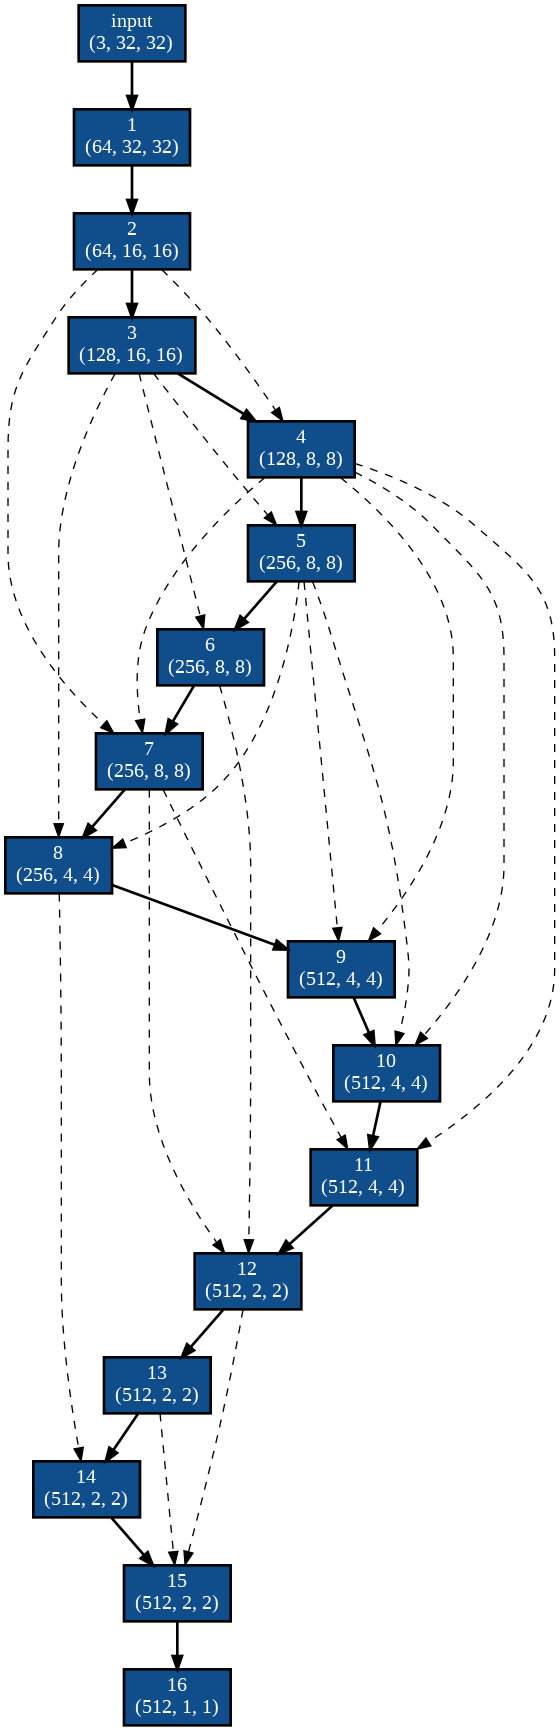
\includegraphics[clip,width=75mm]{graph_50.png}
		\caption{探索したグラフ(50 epoch)}
		\label{fig:search}
	\end{center}
\end{figure*}

\begin{figure*}[tb]
	\begin{center}
		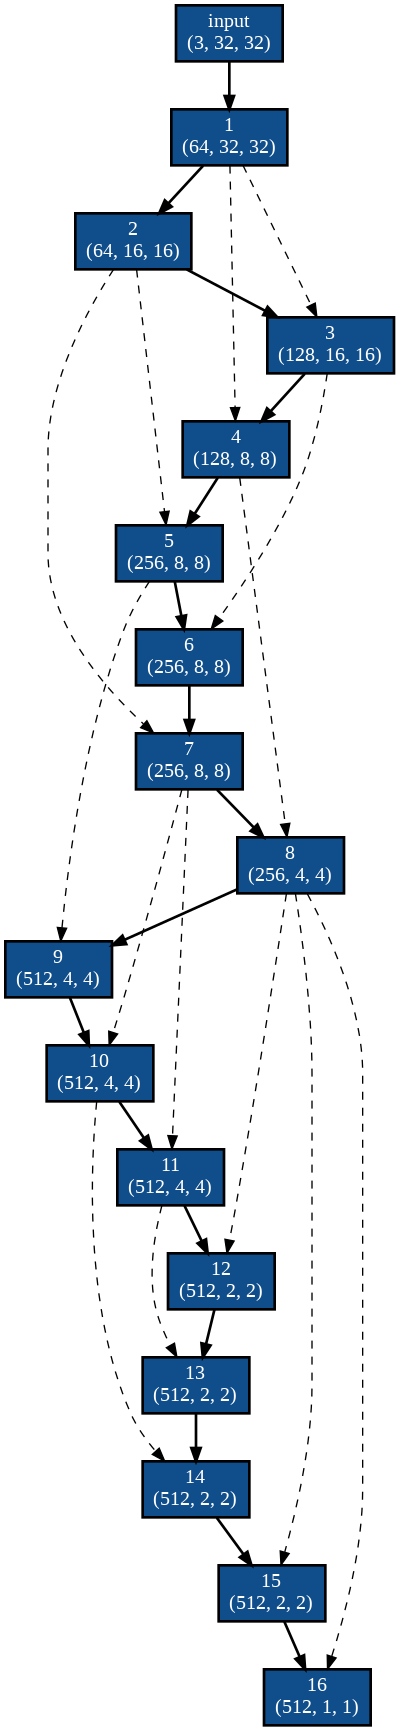
\includegraphics[clip,width=50mm]{graph_1.png}
		\caption{未探索のグラフ(0 epoch)}
		\label{fig:search_no}
	\end{center}
\end{figure*}

表\ref{tab:acc}に結果を示した.
ベースラインは下回らなくなった.
% 探索時の$\beta$の重みを整数にしている
さらに精度を高めるには, 1としているショートカットの重みが探索時のものを引き継ぐ形式が考えられる.

図\ref{fig:beta}には, ブロックごとの$\hat{\beta}$の重みを, 図\ref{fig:search}は得られたグラフを示した. 図\ref{fig:search_no}の初期状態から複数本とるか, 取らないかなどの選択が行えていることが分かる.
Block 13, 14の重みが少ないのは, 重みの大きいBlock 15から参照されているため, Block 12とのバラエティを保っていると考えられる.

\section{今後の予定}
% なんとなくなんかの勉強をするとかではなく具体的に

\begin{itemize}
  \item ショートカット関数の改善
  \item $\beta$周りの改良
\end{itemize}

\section{ソースコード}
% 埋め込みでもGitでもいいので参照できるように
githubのnotebookリポジトリ参照

% 参考文献リスト
\bibliographystyle{unsrt}
\bibliography{ref}
\end{document}
